\documentclass{beamer}
\mode<presentation>
\usetheme{CambridgeUS}
\usepackage[russian]{babel}
\usepackage[utf8]{inputenc}
\usepackage[T2A]{fontenc}
\usepackage{sansmathaccent}

\usepackage{verbatim}
\usepackage{alltt}

\pdfmapfile{+sansmathaccent.map}
\title[Итерционные методы]{Итерационные методы}
\author{Наумов Д.А., доц. каф. КТ}
\date[31.10.2019] {Программирование и алгоритмические языки, 2019}

\begin{document}

%ТИТУЛЬНЫЙ СЛАЙД
\begin{frame}
  \titlepage
\end{frame}
  
%СОДЕРЖАНИЕ ЛЕКЦИИ
\begin{frame}
  \frametitle{Содержание лекции}
  \tableofcontents  
\end{frame}

\section{Циклические алгоритмы}

\begin{frame}{Итерационные методы}
\begin{block}{Итерационные методы}
методы приближенного решения задач прикладной математики, основанные на последовательном приближении к решению путем многократного применения какой-либо вычислительной процедуры.
\end{block}
В данной теме итерационные алгоритмы используются при:
\begin{itemize}
\item вычислении функций с использованием рядов;
\item уточнении корней уравнений;
\item численном интегрировании.
\end{itemize}
\end{frame} 

\begin{frame}{Итерационные методы}
Общая схема итерационного процесса:
\begin{figure}[h]
\centering
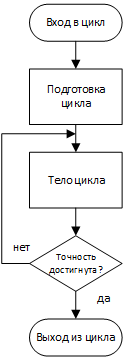
\includegraphics[scale=0.75]{images/lec05-pic01.png}
\end{figure}
\end{frame} 

\begin{frame}{Итерационные методы}
Из-за различных ошибок
\begin{itemize}
\item ошибок ввода исходных данных;
\item ошибок программирования;
\item ошибок времени выполнения; 
\end{itemize}
могут возникать зацикливания – \textbf{бесконечно повторяемые вычисления}
\end{frame}

\begin{frame}
Схема итерационного процесса с ограничением количества итераций:
\begin{figure}[h]
\centering
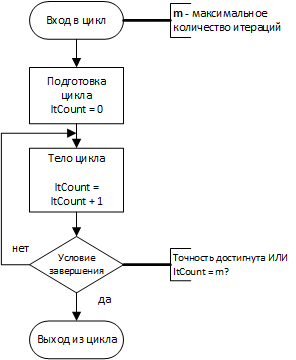
\includegraphics[scale=0.75]{images/lec05-pic02.png}
\end{figure}
\end{frame} 

\begin{frame}{Итерационные методы}
\begin{itemize}
\item Максимальное число итераций \textit{m} должно гарантировать достижение заданной точности вычислений. 
\item Фактическое число повторений цикла определяется величиной допустимой погрешности, а не значением \textit{m}. 
\item Если в теле цикла или в проверяемом условии будут ошибки, приводящие к зацикливанию, то повторения будут
прекращены при достижении счетчиком итераций ItCount предельного значения.
\end{itemize}
\end{frame}

\begin{frame}{Вычисление суммы ряда}
При вычислении значения функции с использованием функционального ряда:
\[\sum\limits_{n=1}^\infty f_n(x)=f_1(x)+f_2(x)+...+f_n(x)\]
задача сводится к последовательному вычислению частичных сумм $S_1(x), S_2(x),..., S_n(x)$, где 
\[S_n(x)=\sum\limits_{i=1}^n f_i(x)\]
Для сходящегося ряда существует предел 
\[\lim\limits_{n\to \infty} S_n(x)=S(x)\]
где $S(x)$ - сумма функционального ряда.
\end{frame}

\begin{frame}
При вычислении суммы ряда с точностью до слагаемого, не превышающего $\varepsilon$, в качестве окончательного результата принимается значение частичной суммы $S_n(x)$, для которой выполняется условие:
\[|f_n(x)<\varepsilon|\]
Процесс вычисления суммы определяется рекуррентным соотношением:
\[S_n(x)=S_{n-1}(x)+f_n(x)\]
\begin{itemize}
\item суммирование считается законченным при выполнении условия достижения заданной точности. 
\item начальное значение суммы принимается равным нулю.
\end{itemize}
В общем случае начальное значение номера члена ряда может быть отличным от единицы (например, равным нулю). Обозначив его через k, получим:
\[S(x)=\sum\limits_{n=k}^\infty f_n(x)\]
\end{frame}

%метод итераций для уточнения корней
%численное интегрирование



\end{document}
